
\subsection{Setup Procedure}

To setup a new authority node read this whole document and then use this procedure to carry out the set up. The full process is shown in Figure ~\ref{fig:onboardflow}

\begin{enumerate}
    \item Choose hosting provider (on-premise or qualified cloud provider) and favored operating system
    \item Consult with EWF NetOps on location and operating system
    \item EWF NetOps will provide the location and OS to use, along with the official installation script for the chosen operating system
    \item Install operating system according to this document
    \item Deploy blockchain node in none-validator mode using the script given by NetOps 
    \item Contact EWF NetOps to confirm installation and incoming telemetry
    \item Create Validator Keys and prepare your node configuration to switch to authority mode using the script.
    \item Send the validator account information to the EWF Governance team
    \item Re-start your node in authority-mode
\end{enumerate}

\begin{figure}[ht]
	\centering
    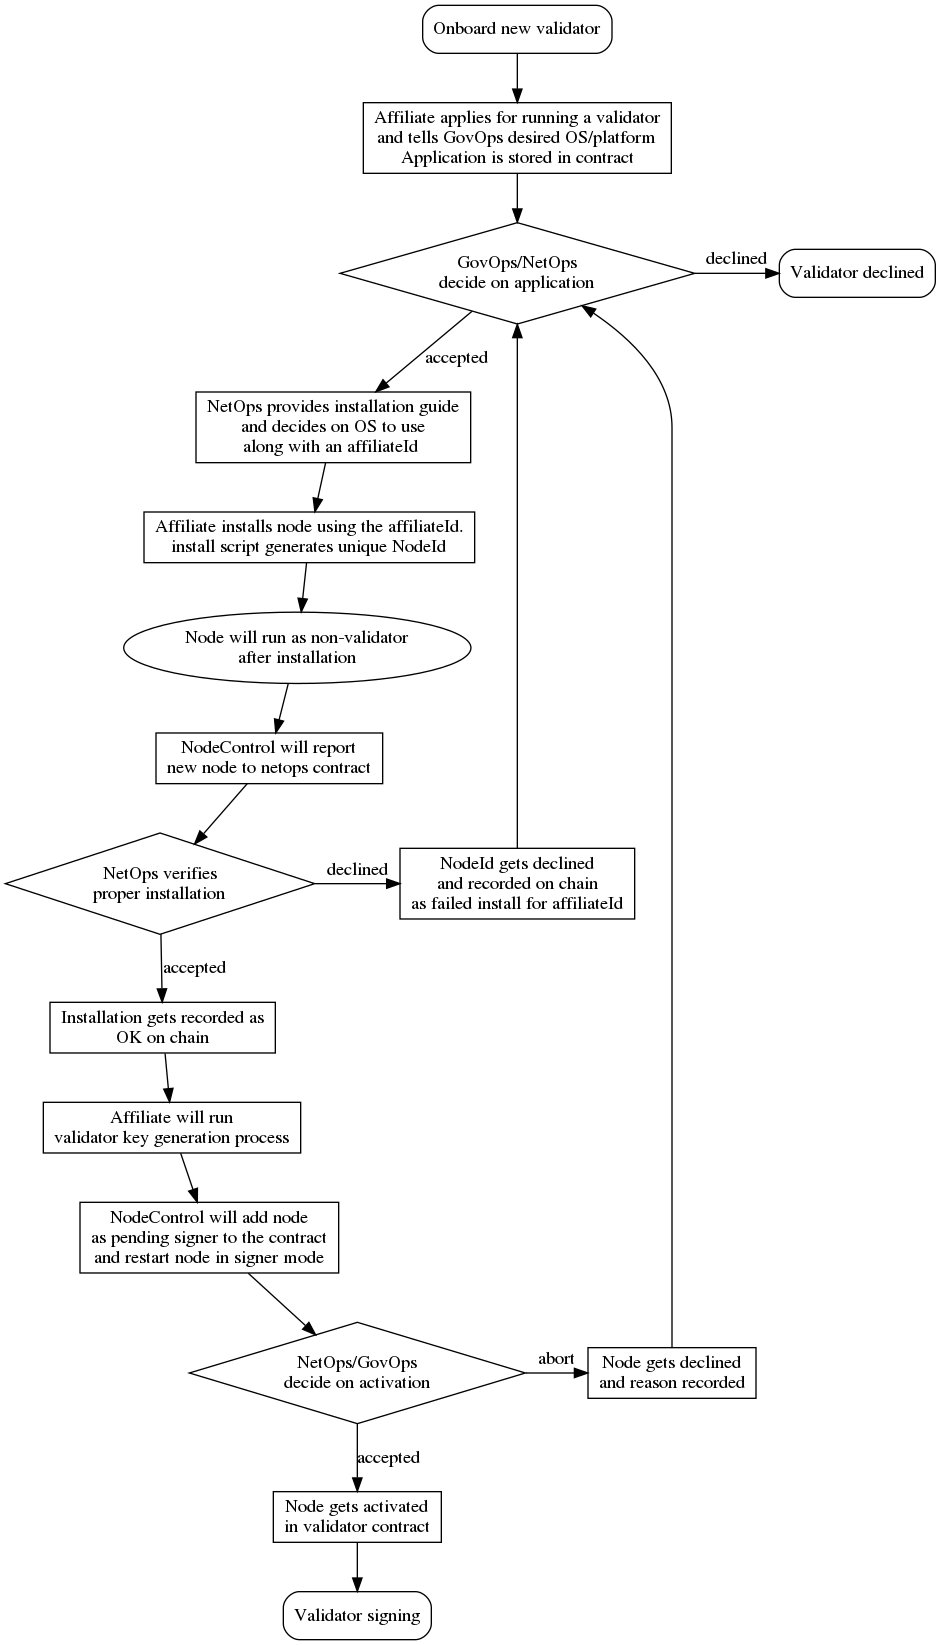
\includegraphics[width=\textwidth,height=\textheight,keepaspectratio]{./images/flow-onboard-validator.png}
	\caption{Validator On-Boarding Flow}
	\label{fig:onboardflow}
\end{figure}
